%\documentclass[openany]{book}
\documentclass[12pt]{article}
\usepackage[utf8]{inputenc}
%\usepackage{amssymb} %for fancy L
%\usepackage{calrsfs} %for fancy L
\usepackage{cancel}
\usepackage{tabularx}
\usepackage[hyphens]{url}
\usepackage{booktabs}
\usepackage{graphicx}
\usepackage[titletoc,title]{appendix}
\usepackage{subfig}
%\DeclareMathAlphabet{\pazocal}{OMS}{zplm}{m}{n} %for fancy L
\usepackage{epsfig, float,array,tabu,longtable,}
\usepackage[hidelinks]{hyperref,wrapfig}
\usepackage{enumerate}
\usepackage{graphicx,psfrag}
\usepackage{cite}
\usepackage{sectsty}
\usepackage{epstopdf}
\usepackage{amsmath,esint, setspace, fancyhdr, amsfonts, bookmark, blindtext}
\usepackage[normalem]{ulem}
\usepackage{tikz}
\usepackage{rotating}
\usepackage[americanvoltages,fulldiodes,siunitx]{circuitikz}
\usepackage{stackengine}
\usetikzlibrary{matrix}
\usepackage{multirow}
\usepackage{multicol}
\usetikzlibrary{shapes,backgrounds,patterns}
\usetikzlibrary{mindmap,trees,decorations.markings}
\usetikzlibrary{quotes,angles}
\usepackage{verbatim}
\renewcommand{\baselinestretch}{1}
\setlength{\textheight}{8in}
\setlength{\textwidth}{6.5in}
\setlength{\headheight}{0in}
\setlength{\headsep}{0.25in}
\usepackage{graphicx}
\setlength{\topmargin}{0in}
\setlength{\oddsidemargin}{0in}
\setlength{\evensidemargin}{0in}
\setlength{\parindent}{.3in}
\usepackage{listings}
\usepackage{color} %red, green, blue, yellow, cyan, magenta, black, white
\definecolor{mygreen}{RGB}{28,172,0} % color values Red, Green, Blue
\definecolor{mylilas}{RGB}{170,55,241}
\doublespacing
\usepackage{pdfpages}
\begin{document}


\begin{titlepage}

\newcommand{\HRule}{\rule{\linewidth}{0.5mm}} % Defines a new command for the horizontal lines, change thickness here

\center % Center everything on the page
 
%---------------------------------------------------------
%	HEADING SECTIONS
%---------------------------------------------------------

\textsc{\LARGE one versus two hour intentional rounding}\\[1.5cm] % Major Heading
\textsc{\Large a pragmatic randomized multiple-crossover trial}\\[0.5cm] % Major heading s
\textsc{\large }\\[0.5cm] % Minor heading

%---------------------------------------------------------
%	TITLE SECTION
%---------------------------------------------------------

\HRule \\[0.6cm]
{ \huge \bfseries Research Protocol}\\[0.4cm] % Title of your document
\HRule \\[1.0cm]
 
%---------------------------------------------------------
%	AUTHOR SECTION
%---------------------------------------------------------

%\begin{minipage}{0.4\textwidth}
\begin{center} \large
% \emph{Authors:}  
\medskip
{\textsc{\textbf{Aaron Conway} }}  \quad  {\textsc{\textbf{Linda Flockhart}}}  \quad {\textsc{\textbf{Zelia Souter}}} \quad {\textsc{\textbf{Dorina Baston}}}\quad {\textsc{\textbf{Monika Kerri}}}\quad {\textsc{\textbf{Miranda Hadzic}}}% Your name, bold and small caps
\end{center}
%\end{minipage}

\begin{center} \Large
{\textsc{\textbf{Version 1 (Draft)} }} 
\end{center}

~
%\begin{minipage}{0.4\textwidth}
%\begin{flushright} \large
%\emph{Supervisor:} \\
%Dr. James \textsc{Smith} % Supervisor's Name
%\end{flushright}
%\end{minipage}\\[4cm]

% If you don't want a supervisor, uncomment the two lines below and remove the section above
%\Large \emph{Author:}\\
%John \textsc{Smith}\\[3cm] % Your name

%---------------------------------------------------------
%	DATE SECTION
%---------------------------------------------------------
\begin{center}
{\large \today}
\end{center}
 % Date, change the \today to a set date if you want to be precise

%---------------------------------------------------------
%	LOGO SECTION
%---------------------------------------------------------
%\vfill

\newcommand*{\plogo}{
\includegraphics[width=0.5\textwidth]{image001.jpg}}

\plogo\\[1cm] % Include a department/university logo - this will require the graphicx package
 
%---------------------------------------------------------

\vfill % Fill the rest of the page with whitespace
\end{titlepage}

\newpage
\tableofcontents
\newpage

% EXECUTIVE SUMMARY %%%%%%%%%%%%%%%%%%%%%%%%%%%%%%%%%%
\section{Summary}
\subsubsection*{Primary Objective}
To compare the effects of performing intentional rounding every one or two hours on patient outcomes. 
\subsubsection*{Study Design}
A pragmatic, randomized, multiple-crossover trial will be conducted. The frequency that nurses perform intentional rounding within participating departments at the Peter Munk Cardiac Centre will be randomly assigned as either one hour or two hours on a monthly basis. All other elements of the rounding process will remain the same.

\subsubsection*{Outcomes}
The primary outcome is the count of falls (reported in the incident reporting system) per 1000 patient days. Secondary outcomes are:
\begin{itemize}
    \item Falls with injuries
    \item Completeness of documentation of intentional rounding
    \item Patient satisfaction 
    \item Call bell requests to nursing staff
    \item \colorbox{yellow}{Missed vital signs?}
    \item \colorbox{yellow}{Nutrition?}
    \item \colorbox{yellow}{Medication errors?}
    \item \colorbox{yellow}{Clinical deterioration (measured as the number of MET calls)?}
    \item \colorbox{yellow}{Pressure injuries?}
\end{itemize}


\subsubsection*{Study Population}
All patients admitted to the Cardiology and Cardiovascular Surgery inpatient wards at the Peter Munk Cardiac Centre. 

\subsubsection*{Sample Size}
The study duration has been set to 12 months and the sample size will be the number of patients admitted to the study wards during that time. This study duration was chosen based on feasibility considerations and to ensure several crossovers, enrollment throughout the year and to accumulate a large sample size adequate to detect important difference in outcomes between groups. Based on historical data from the Peter Munk Cardiac Centre, we anticipate a sample size of approximately \colorbox{yellow}{6000} patients distributed between the \textit{one-hour} and \textit{two-hour} hour intentional rounding groups.


\section{Background}
Intentional rounding is being implemented in healthcare settings across the globe. It has been stated that more than 400 healthcare systems in the United States has implemented intentional rounding usinng the methods outlines by the Studer Group.\cite{studer2007} In the United Kingdom, the NHS has  from the Francis report and in the US to improve patient satisfaction)\cite{francis2013report}

Bibliometric analysis of the published literature clearly demonstrate the increasing popularity of intentional rounding.\cite{hutchinson2017mapping} In the period between 2005 and 2015, there has been 38 separate studies published that evaluated some form on intentional rounding. A predominance of these studies has originated from the United States. \textit{Scripted} or \textit{structured} rounding dominated the literature as the most common method used to implement rounding. Several recent systematic reviews that have assessed the quality of studies that examined the effect of intentional rounding on patient outcomes have all highlighted the important point that further higher quality studies are required.\cite{christiansen2018intentional, toole2016systematic, hutchinson2017mapping, sims2018realist, flowers2016intentional} 

Addressing the  intentional rounding \textit{evidence-void}, as it has been described by Hutchinson et al \cite{hutchinson2016intentional}, is vital. There have been \textbf{no} randomized trials conducted to evaluate either the effectiveness of intentional rounding in general or for specific components of how intentional rounding is implemented. Unfortunately this is not a unique situation for critical nursing interventions. For example, Cochrane reviews examining core nursing practices such as the effectiveness of repositioning for pressure ulcer reduction \cite{gillespie2014repositioning} and nursing handover processes\cite{lockwood2016best} identified only few studies. Richards et al\cite{richards2018fundamental} conducted a comprehensive systematic review that aimed to identify experimental studies examining the effects of nursing interventions for people's nutrition, elimination mobility and hygiene needs, which were deemed as \textit{fundamental nursing care}. Of 149 studies identified, all but 13 were low quality with significant risk of bias. Addressing this lack of evidence to inform core aspects of nursing care interventions in hospitals is achievable. Innovative research designs that incorporate strategies to minimize risk of bias when studying the effectiveness of alternative approaches to nursing care should be utilized. One way to accomplish this is to incorporate randomization into standard care so that routine data collected can be measured to compare the effectiveness of alternative approaches to nursing care. 

Based on this prior evidence, it is reasonable to hypothesize that there may be differences in patient outcomes between the frequency that intentional rounding is performed by nurses. 

-UHN context regarding implementation of intentional rounding\\
-Outcomes that intentional rounding is thought to influence and mechanisms (i.e. falls, patient satisfaction)\\
-Variation in components of intentional rounding (structured/unstructured, frequency, components, documentation)\\


The completeness of documenting that all elements of intentional rounding has been shown to be poor.\cite{tucker2012outcomes}

-Limitations in the evidence\\

-Potential for adverse or unintended consequences to arise from implementation of intentional rounding. For example, a prominent finding reported in a realist synthesis of the literature about intentional rounding was that  nurses have explained that intentional rounding activities took up more time for complex and demanding patients, which consequently prioritized their needs over others.\cite{sims2018realist}

\section{Objective}
To compare the effects of performing intentional rounding every one or two hours on patient outcomes. 

\section{Methods}

A pragmatic, randomized multiple-crossover trial will be conducted. Numerous short periods with frequent crossovers was selected to minimize the risk of changes over time in the patient population and usual care confounding trial results. The approach of using multiple crossovers in a pragmatic trial to compare the effects of standard treatments applied in clinical practice is established and has been previously used, including a high profile study recently published in the New England Journal of Medicine.\cite{self2018} 


We decided that it is suitable to compare the effects of different frequencies of intentional rounding using a multiple crossover design because there is no risk of carryover effects. Intentional rounding will only have an effect on patient outcomes at the time it is being applied. Furthermore, compared with the prior observational studies conducted to evaluate the efficacy of intentional rounding, our trial design incorporates a randomization procedure to reduce risk of bias.

\subsection{Population}
The trial will be conducted at the Toronto General Hospital, a tertiary care academic hospital with 432 beds in Toronto, Canada. The study population includes inpatients in the participating wards of the Peter Munk Cardiac Centre. Inpatient units from the Peter Munk Cardiac Centre will participate. The cardiovascular surgery inpatient unit comprises two separate wings with a population comprising patients diagnosed with a heart disease requiring surgery such as coronary artery bypass grafting, valvular repair/replacement and adult congenital heart repair. The cardiology inpatient unit serves a population of patients with a heart condition including acute coronary syndrome, cardiac arrhythmia, cardiomyopathy and heart failure. The cardiac short stay unit serves primarily cardiac patients who are undergoing procedures that require admission to hospital for less than 2 days.  The study period will be from 01 August 2019 to 31 July 2020.



\subsection{Intervention and control conditions}
The University Health Network hospital departments that implement intentional rounding utilize a framework to ensure that the structure of rounding is focused on the patient experience. There are 6 major elements to be incorporated by the nurse in each instance of intentional rounding. These elements along with specific actions to be performed and their rationale are outlined in Figure \ref{fig1}. 

\begin{figure}[ht]
\centering
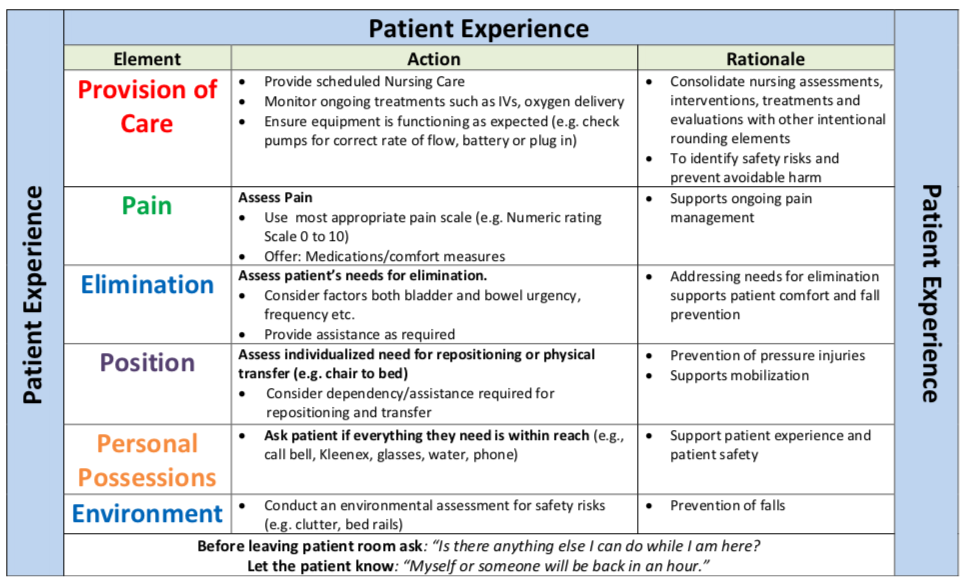
\includegraphics[width=\textwidth]{IRelements.png}
\caption{Intentional Rounding Elements}
\label{fig1}
\end{figure}

The frequency of intentional rounding for the study periods will be communicated to nurses in several ways to ensure they adhere to the assigned conditions for the trial. These include:
\begin{itemize}
    \item Bedside reminders
    \item Direct communication reminder at safety huddles
    \item \colorbox{yellow}{need more info in this section}
\end{itemize}


\subsubsection{One hour intentional rounding}
Intentional rounding during the months assigned \textit{one-hour} frequency should be performed at least once every hour throughout the day and night. 

\subsubsection{Two hour intentional rounding}
Intentional rounding during the months assigned \textit{two-hour} frequency should be performed at least once every two hours throughout the day and night. 

\subsection{Outcomes}

\subsubsection{Primary}
We define a fall as an event that results in an individual coming to rest inadvertently on a lower level, with or without injury.

\subsubsection{Secondary}

\begin{itemize}
    \item \textit{Fall injury}\\
    A fall injury is defined as an injury that results from a fall, which may or may not require treatment. The injury can be temporary or permanent and vary in the severity of harm. Fall injuries will be categorized as minor, moderate or severe, according to the hospital classification system.
    
    \item \textit{Completeness of documentation of intentional rounding}\\
    Log sheets have been developed by UHN for nurses to document which elements of intentional rounding have been performed. There is a checkbox for: .... (An example of the log sheet is provided in Section \ref{AppA}: Appendix A). The proportion of intentional rounding log sections completed at each rounding occurrence will be calculated. The proportion of rounding logs completed over a 24-hour period relative to the frequency of intentional rounding assigned to the randomization period (i.e. every one or two hours) will also be calculated. A composite of these two measures will also be calculated, being the proportion of the the total number of intentional rounding sections completed over the 24-hour period.
    \item \textit{Patient satisfaction} \\
    Previous research found that rounding increased satisfaction across all subscales of  Hospital Consumer Assessment of Healthcare Providers and Systems.\cite{brosey2015effectiveness} 
    \item Call bell requests to nursing staff
    \item Medication Errors?
    \item Nutrition?
    \item Clinical deterioration (measured as the number of MET calls)?
     \item \colorbox{yellow}{Pressure injuries?}
\end{itemize}


\subsection{Procedures}



\subsubsection{Enrollment}
All patients admitted to participating wards will be included unless they elect to 'opt-out' of having their data included in the study. An information letter will be provided to all in-patients in participating wards, explaining the study. If the patient elects to 'opt-out' they will be asked to complete a withdrawal of consent form and return it to the nursing staff.

\subsubsection{Randomization sequence generation and allocation concealment}
A statistician will generate a randomization sequence to assign the frequency for intentional rounding for each month of the calendar year. The treatment assignment will be communicated to Nurse Managers the week prior to the start of each month so that staff can be informed of the frequency that intentional rounding is to be performed. Concealing the allocation until this time may reduce risk of bias associated with anticipatory changes in nurse staffing depending on the upcoming allocation. 

\subsubsection{Data collection}
Data about the demographics of the patients admitted to participating wards during the study period will be collected from the Electronic Patient Record. Data on outcomes that are routinely collected (i.e. falls) will be collected from the Electronic Patient Record and the hospital Incident Reporting System. Data used in this study that are not routinely collected (such as call bell usage and patient satisfaction scores) will be collected by a trained Research Coordinator using electronic Case Report Form designed in REDCap.

\subsection{Instruments}

\subsubsection{Incident reporting system}
The hospital incident reporting system will be accessed to calculate the number of falls that occurred in the participating wards during the study period. 


\subsubsection{Canadian Patient Experience Survey - Inpatient Care}
The Canadian Patient Experience Survey for inpatient care (CPES-IC) will be used to measure patient experience. This survey was developed by the Canadian Institute of Health Information. It combines items from the Hospital Consumer Assessment of Healthcare Providers and Systems (HCAHPS) survey as well as item that address key areas relevant to the Canadian in-patient healthcare context. 

An electronic case report form will be designed in REDCAP with fields entered for each item included in the CPES-IC.

Could use the Patient Satisfaction with Nursing Care Quality Questionnaire.\cite{laschinger2005}

*On one randomly selected day per month at each participating ward, all patients scheduled for discharge will be invited to complete a patient experience survey unless they meet the following exclusion criteria:
\begin{itemize}
    \item Duration of hospital admission spanned more than one randomization period (i.e two calendar months)
    \item Was admitted to a department in the Toronto General Hospital not participating in the study at any time during the current hospital admission 
\end{itemize}

\subsubsection{Completeness of intentional rounding documentation}
An electronic case report form was designed in REDCAP with fields entered to capture the completeness of documentation about intentional rounding. A research coordinator will review the intentional rounding logs for 10 randomly selected patients on one randomly selected day each month in each of the participating wards. 


\subsubsection{Electronic patient record}
 Data about the demographic characteristics of the patients admitted to participating wards will be collected using queries of the electronic patient record. 

\subsubsection{Call bell usage audit}
An electronic case report form was designed in REDCAP with fields entered to capture the number of times per hour that a call bell is used in participating wards. A research coordinator will undertake one hour-long audit on one randomly selected day each month in each of the participating wards. The time for the audit will be randomly selected between 0600 and 2200 hours.

Measurements:
\begin{itemize}
    \item Number of calls
    \item Time to attendance (calculated as the difference between the onset and offset of the call bell alert)
\end{itemize}

\subsection{Sample size considerations}
The study duration has been set to 12 months and the sample size will be the number of patients admitted to the participating wards during that time. This study duration was chosen based on feasibility considerations and to ensure numerous crossovers, enrollment throughout the calendar year as well as to accumulate a large sample size adequate to detect important difference in outcomes between groups. Based on historical data from the Peter Munk Cardiac Centre, we anticipate a sample size of approximately \colorbox{yellow}{6000} patients distributed between the \textit{one-hour} and \textit{two-hour} intentional rounding groups.

Due to the current lack of established statistical methodologies for calculating sample size for multiple cross over trials with count outcome variables, we have not performed any sample size calculations for this study. However, the data obtained in this study could be used to facilitate modelling of sample size requirements for a larger scale study across multiple sites.


\subsection{Statistical analysis plan}
 The primary analysis will be an intention-to-treat analysis of eligible patients assigned to one versus two hour intentional rounding based on the primary outcome of falls per 1000 days in hospital. An unadjusted incidence rate ratio, expressed as rate of falls per 1000 patient days in the one hour frequency periods/rate of falls per 1000 patient days in the two hour frequency period, will be calculated using poisson regression. An adjusted analysis will also be conducted to account for the following baseline characteristics: Age, sex, days elapsed since admission and admitting ward. 
 
 \subsubsection{Unit of analysis issues}
 Some patients included in our study will have been admitted in a participating ward for a duration that spanned across more than one crossover period. It is also possible that patients will have been admitted to a ward in the Toronto General Hospital for a period of time during the admission that is not participating in the study. For the majority of outcomes in this trial, including the primary outcome of the number of falls, this is not an issue because there is no carryover effect of the intervention and the outcome will be counted only while the intervention is implemented. For example, consider hypothetically that the randomization sequence was such that patients in the participating wards would receive \textit{one-hour} intentional rounding in the month of May and \textit{two-hour} intentional rounding during the month of June. If a patient admitted to a participating ward had one fall in May and two falls in June, this would be included in the analysis as one fall for the \textit{\textit{one-hour}} group and two falls for the \textit{two-hour} group. 
 The instrument to be used to measure patient satisfaction (CPES-IC) asks patients to rate their degree of satisfaction with different aspects of their hospital care throughout their admission. For this reason, patients whose hospitalization spans only one randomization period and is admitted solely to a participating ward will be included for the analysis of this outcome. 
 
 \section{Ethical considerations}
 
This study employs a novel design to determine the relative efficacy of two standard approaches to the implementation of intentional rounding. As such, it is an \textbf{\textit{interventional}} study. However, many features of the trial are more similar to an \textbf{\textit{observational}} study. Specifically, the study involves only standard care approaches delivered at differing frequencies. In this study, whether a patient will receive intentional rounding at either a one hour or two hour frequency will depend (randomly) on the time of their admission during the year. 

All patients will receive standard care except that the default frequency in which intentional rounding will be performed will be randomly allocated according to the month in which they are admitted to a participating ward in the Peter Munk Cardiac Centre. At present, the frequency of intentional rounding is allocated will vary according to the particular hospital that patients attend. As a result of these factors, this study involved negligible risk. 

The study design will provide high quality information about an important clinical question from a very large number of subjects in a short period of time. It will inform clinical practice much more rapidly than would be possible with a standard randomized controlled trial. Given the low risk nature of the research, we will provide written information to participants about the study on admission to a participating ward and will provide an opportunity for \textit{opt-out} consent from the use of data related to their hospital admission if they wish. 
 
\section{Funding}
This study will be fully supported by funds received by the Principal Investigator, Aaron Conway, for his appointment as Chair of Cardiovascular Nursing Research at PMCC.

% BIBLIOGRAPHY %%%%%%%%%%%%%%%%%%%%%%%%%%%%%%%%%%%%%%%
\newpage
\section{References}

\bibliographystyle{unsrt}
\bibliography{bibliography}
\fancyhead[R,OL]{bibliography}

\begin{appendices}

% APPENDIX A %%%%%%%%%%%%%%%%%%%%%%%%%%%%%
\newpage
\section{Intentional Rounding Log}
\label{AppA}

% APPENDIX B %%%%%%%%%%%%%%%%%%%%%%%%%%%%%
\newpage
\section{Patient Experience Survey}
\begin{itemize}
    \item Canadian Patient Experiences Survey 
\end{itemize}
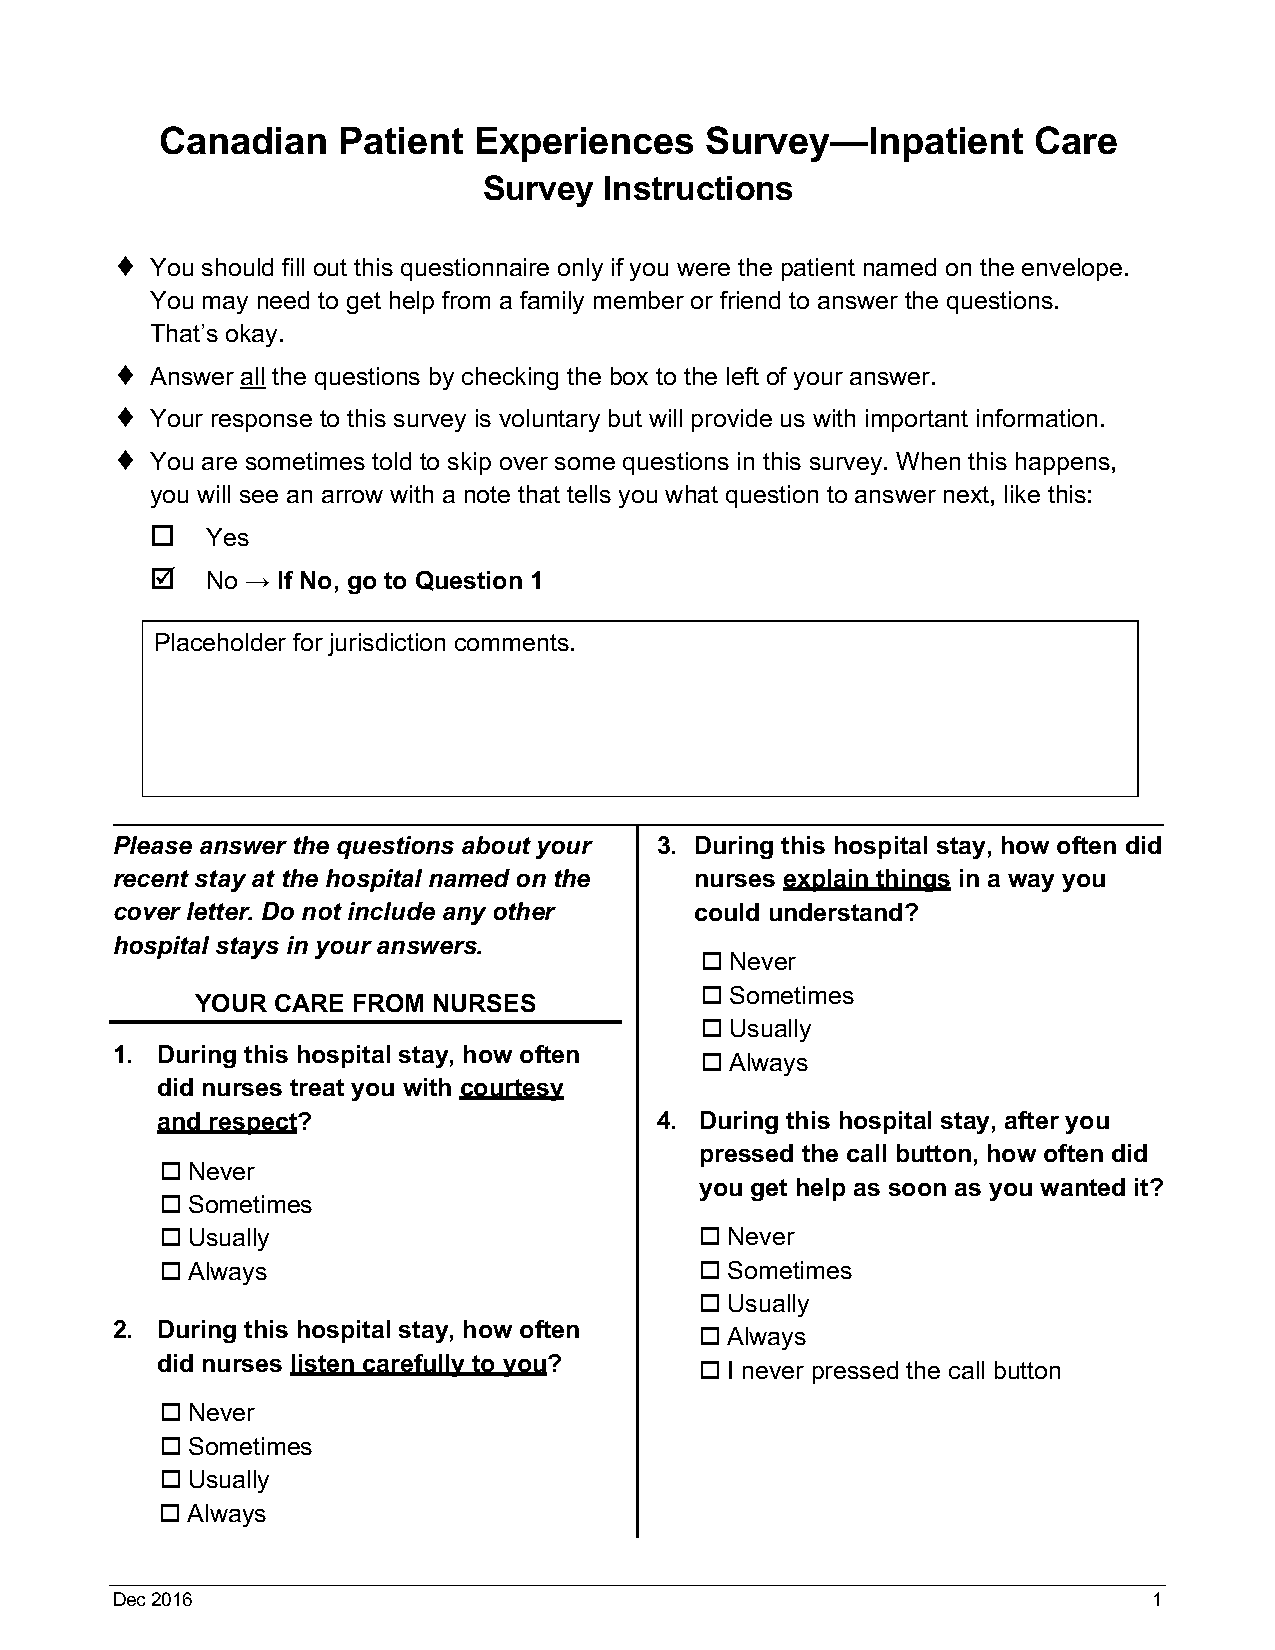
\includepdf[pages={1-},scale=0.75]{CPES-IC.pdf}

\label{AppB}

% APPENDIX C %%%%%%%%%%%%%%%%%%%%%%%%%%%%%
\newpage
\section{Call bell usage case report form}
\label{AppC}

% APPENDIX D %%%%%%%%%%%%%%%%%%%%%%%%%%%%%
\newpage
\section{Intentional rounding documentation case report form}
\label{AppD}

\end{appendices}
\end{document}
